\providecommand{\main}{../../../..}
\documentclass[\main/dresen_thesis.tex]{subfiles}

\begin{document}
  These combinations were also transferred to various other oleic acid ligated nanoparticles during this work, such as cobalt ferrite nanospheres or iron oxide nanocubes as exemplary shown in \reffig{fig:monolayers:preparation:solventVariation:spheresIron}.
  From varied success rates during the transfer to other nanoparticles it became apparent that the oleic acid content within the dispersion is also a crucial part for the monolayer formation, especially for particles synthesized following the acetylacetonate route.

  \begin{figure}[tb]
    \centering
    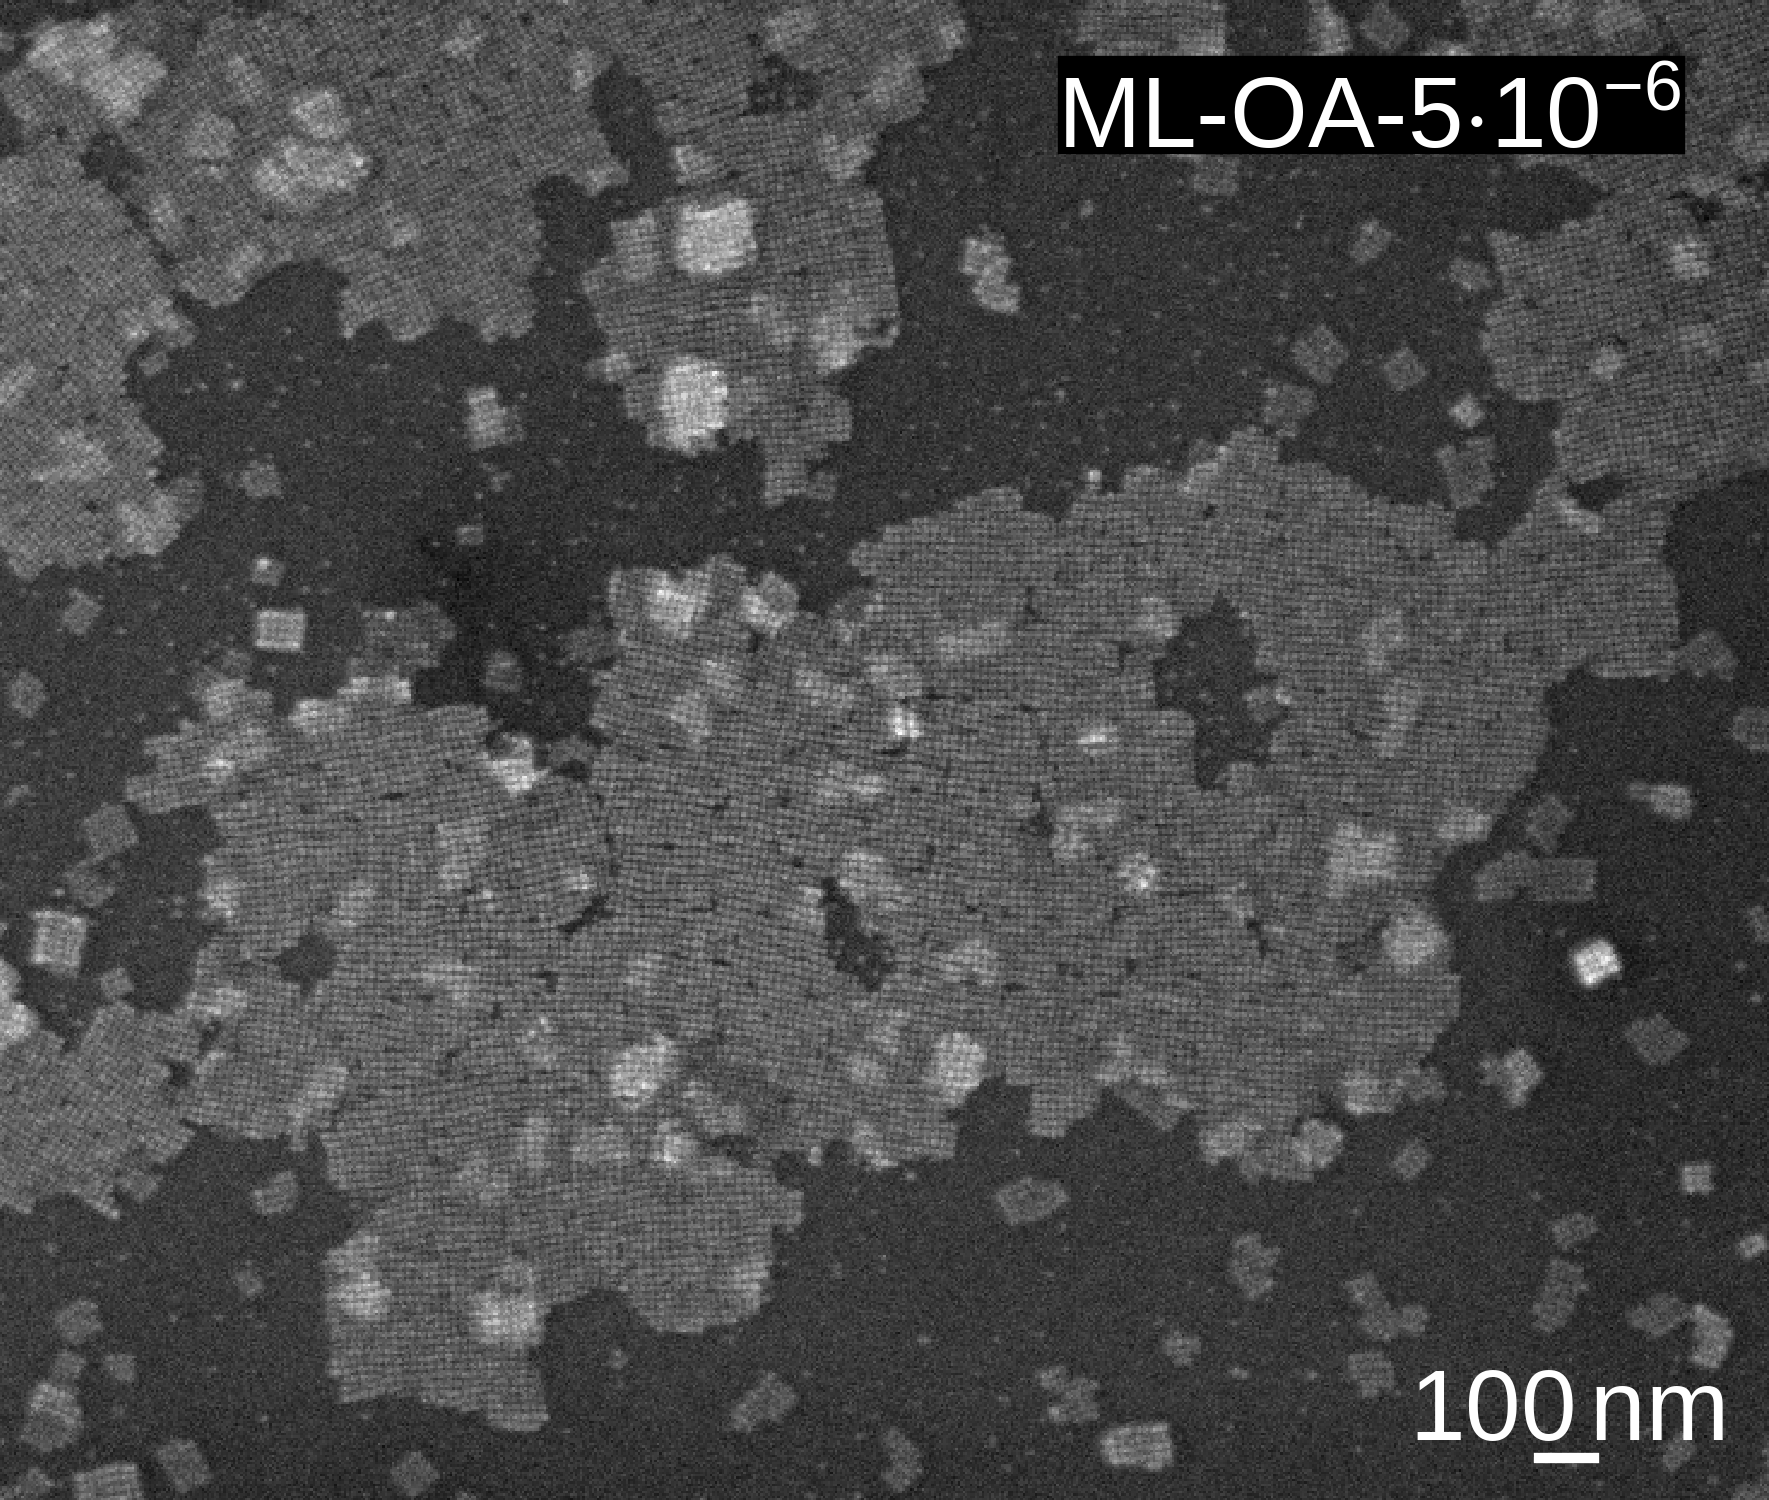
\includegraphics{monolayers_SEM_ML-OA-5e-6}
    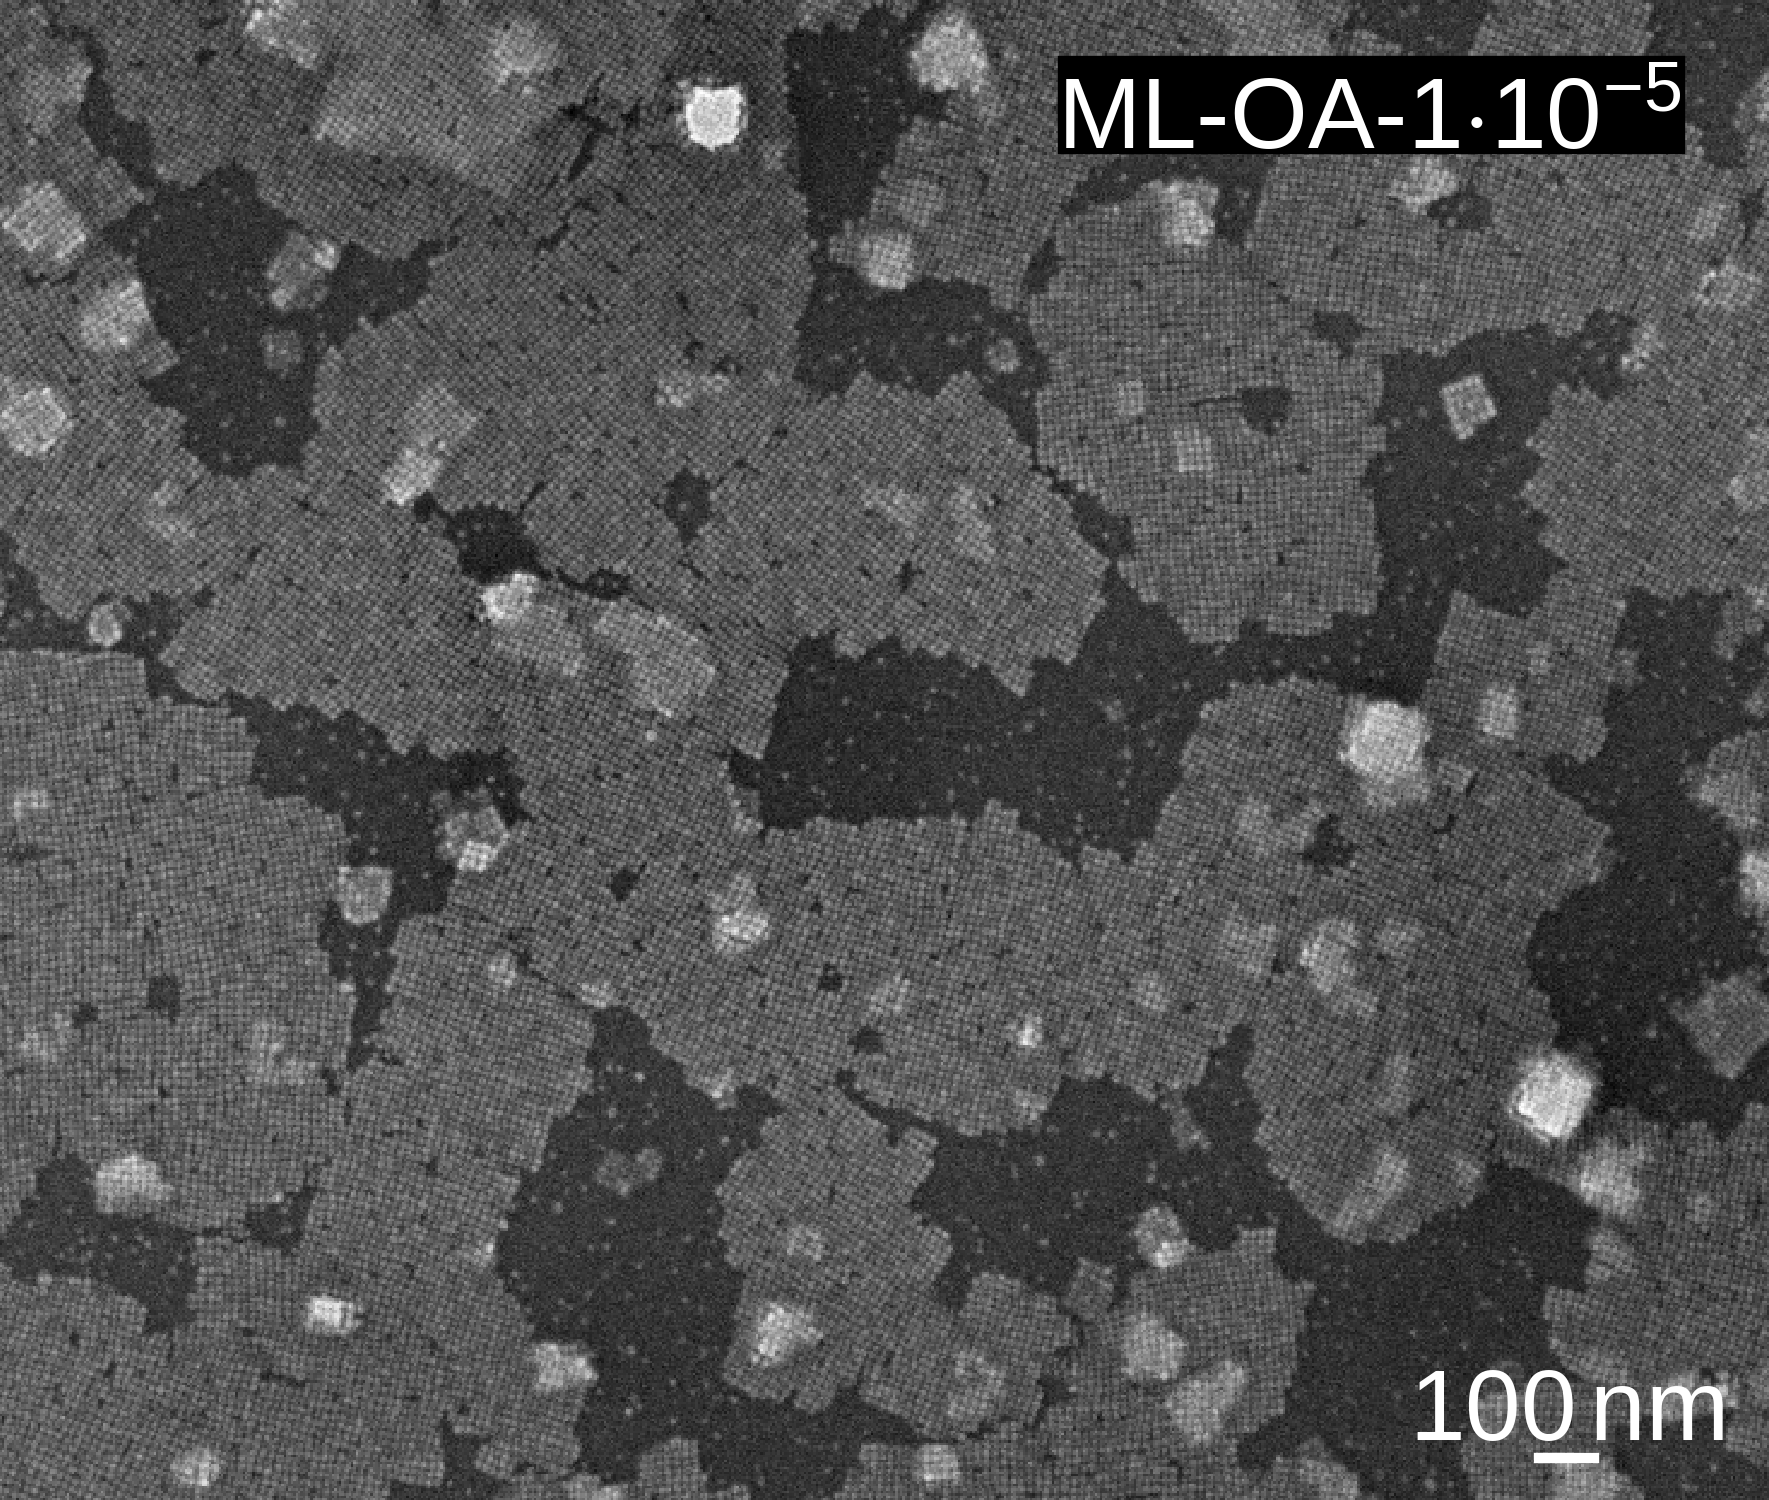
\includegraphics{monolayers_SEM_ML-OA-1e-5}
    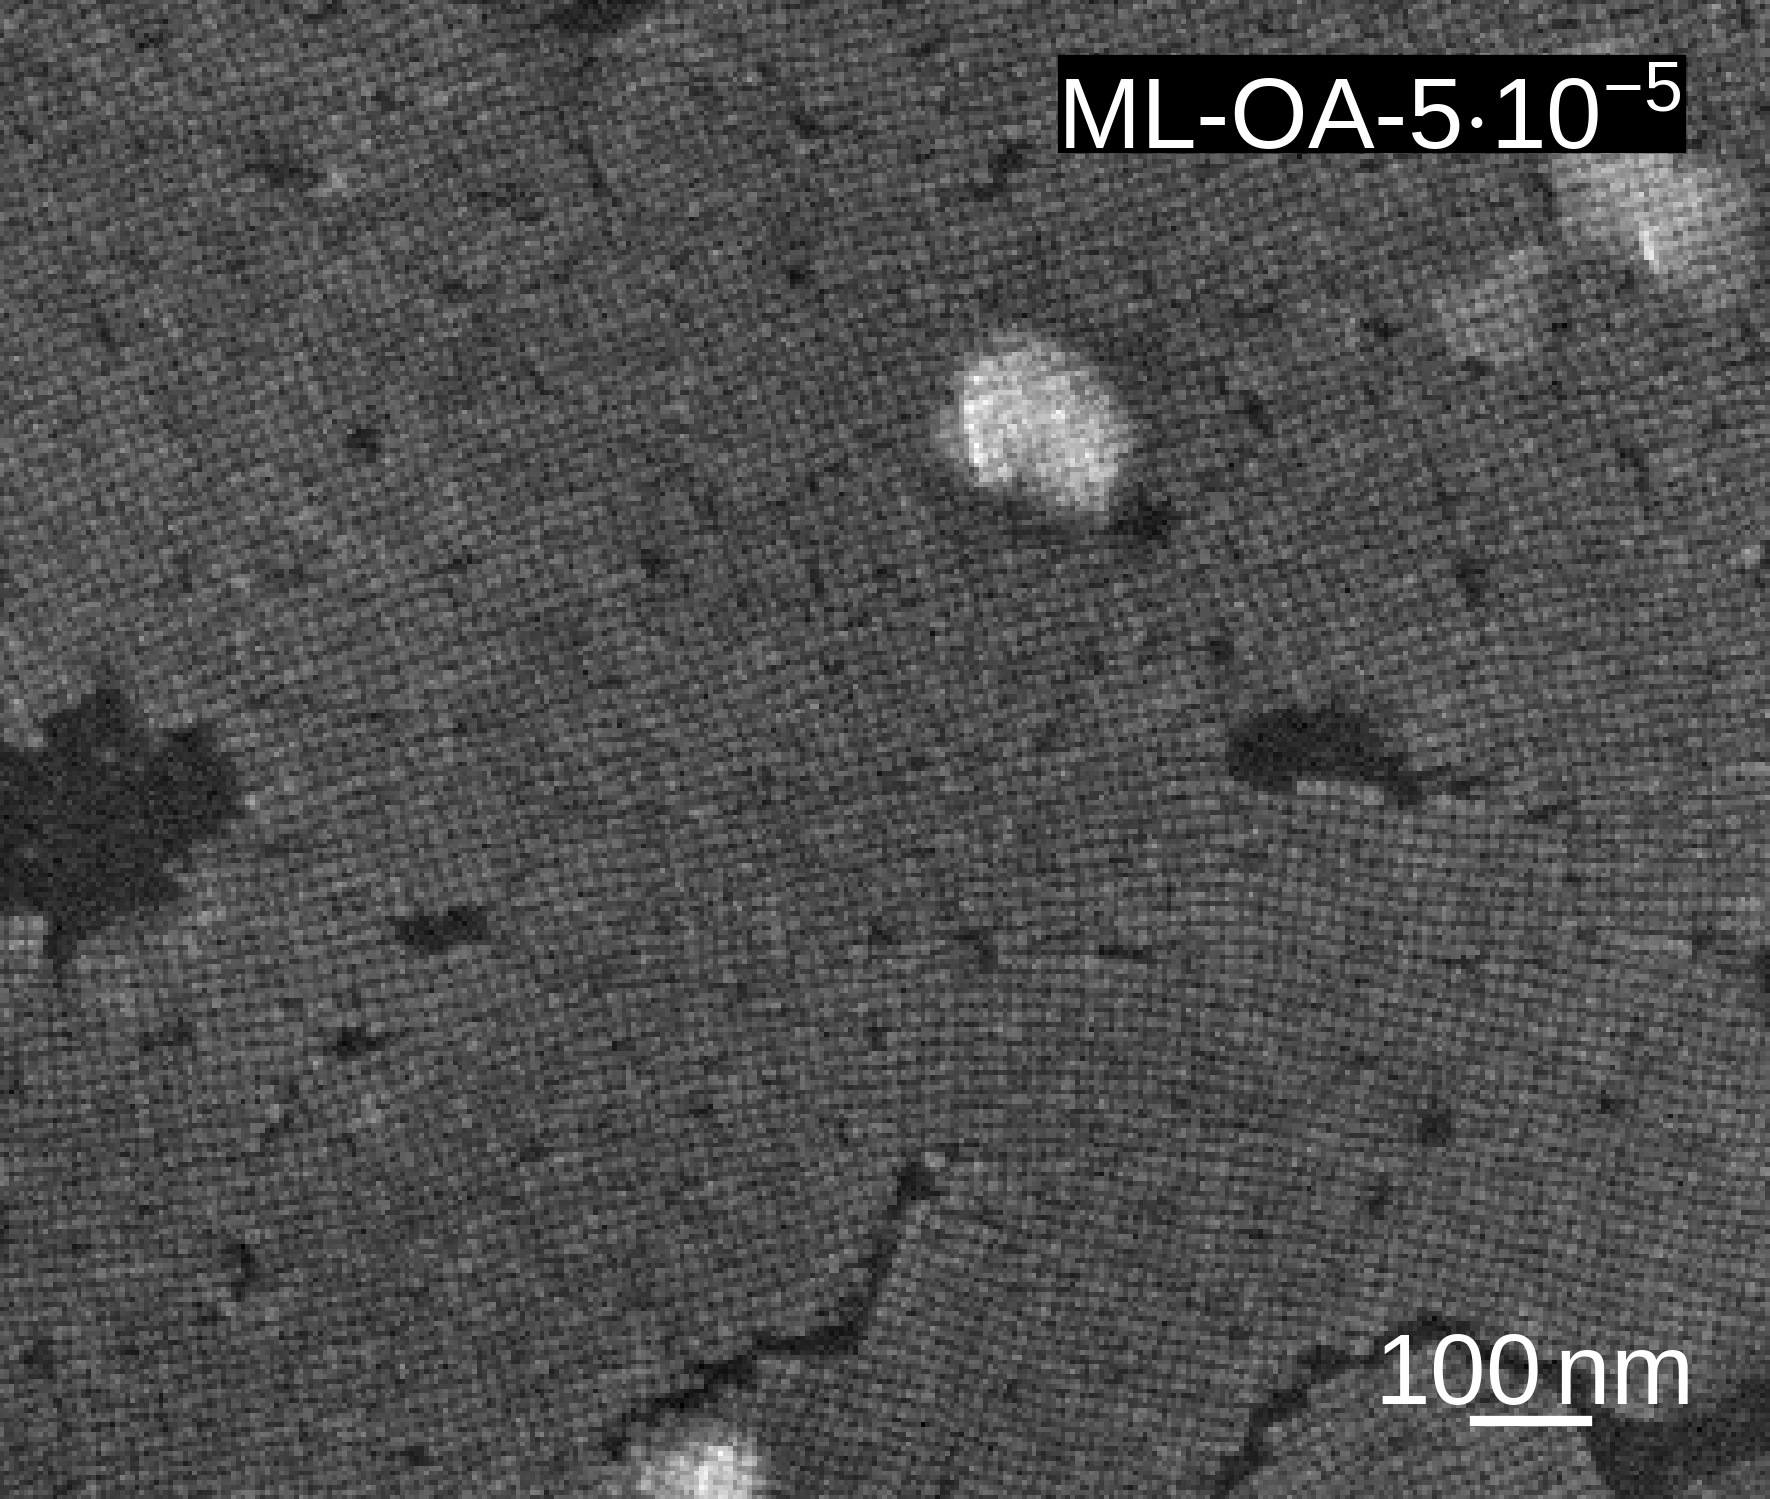
\includegraphics{monolayers_SEM_ML-OA-5e-5}
    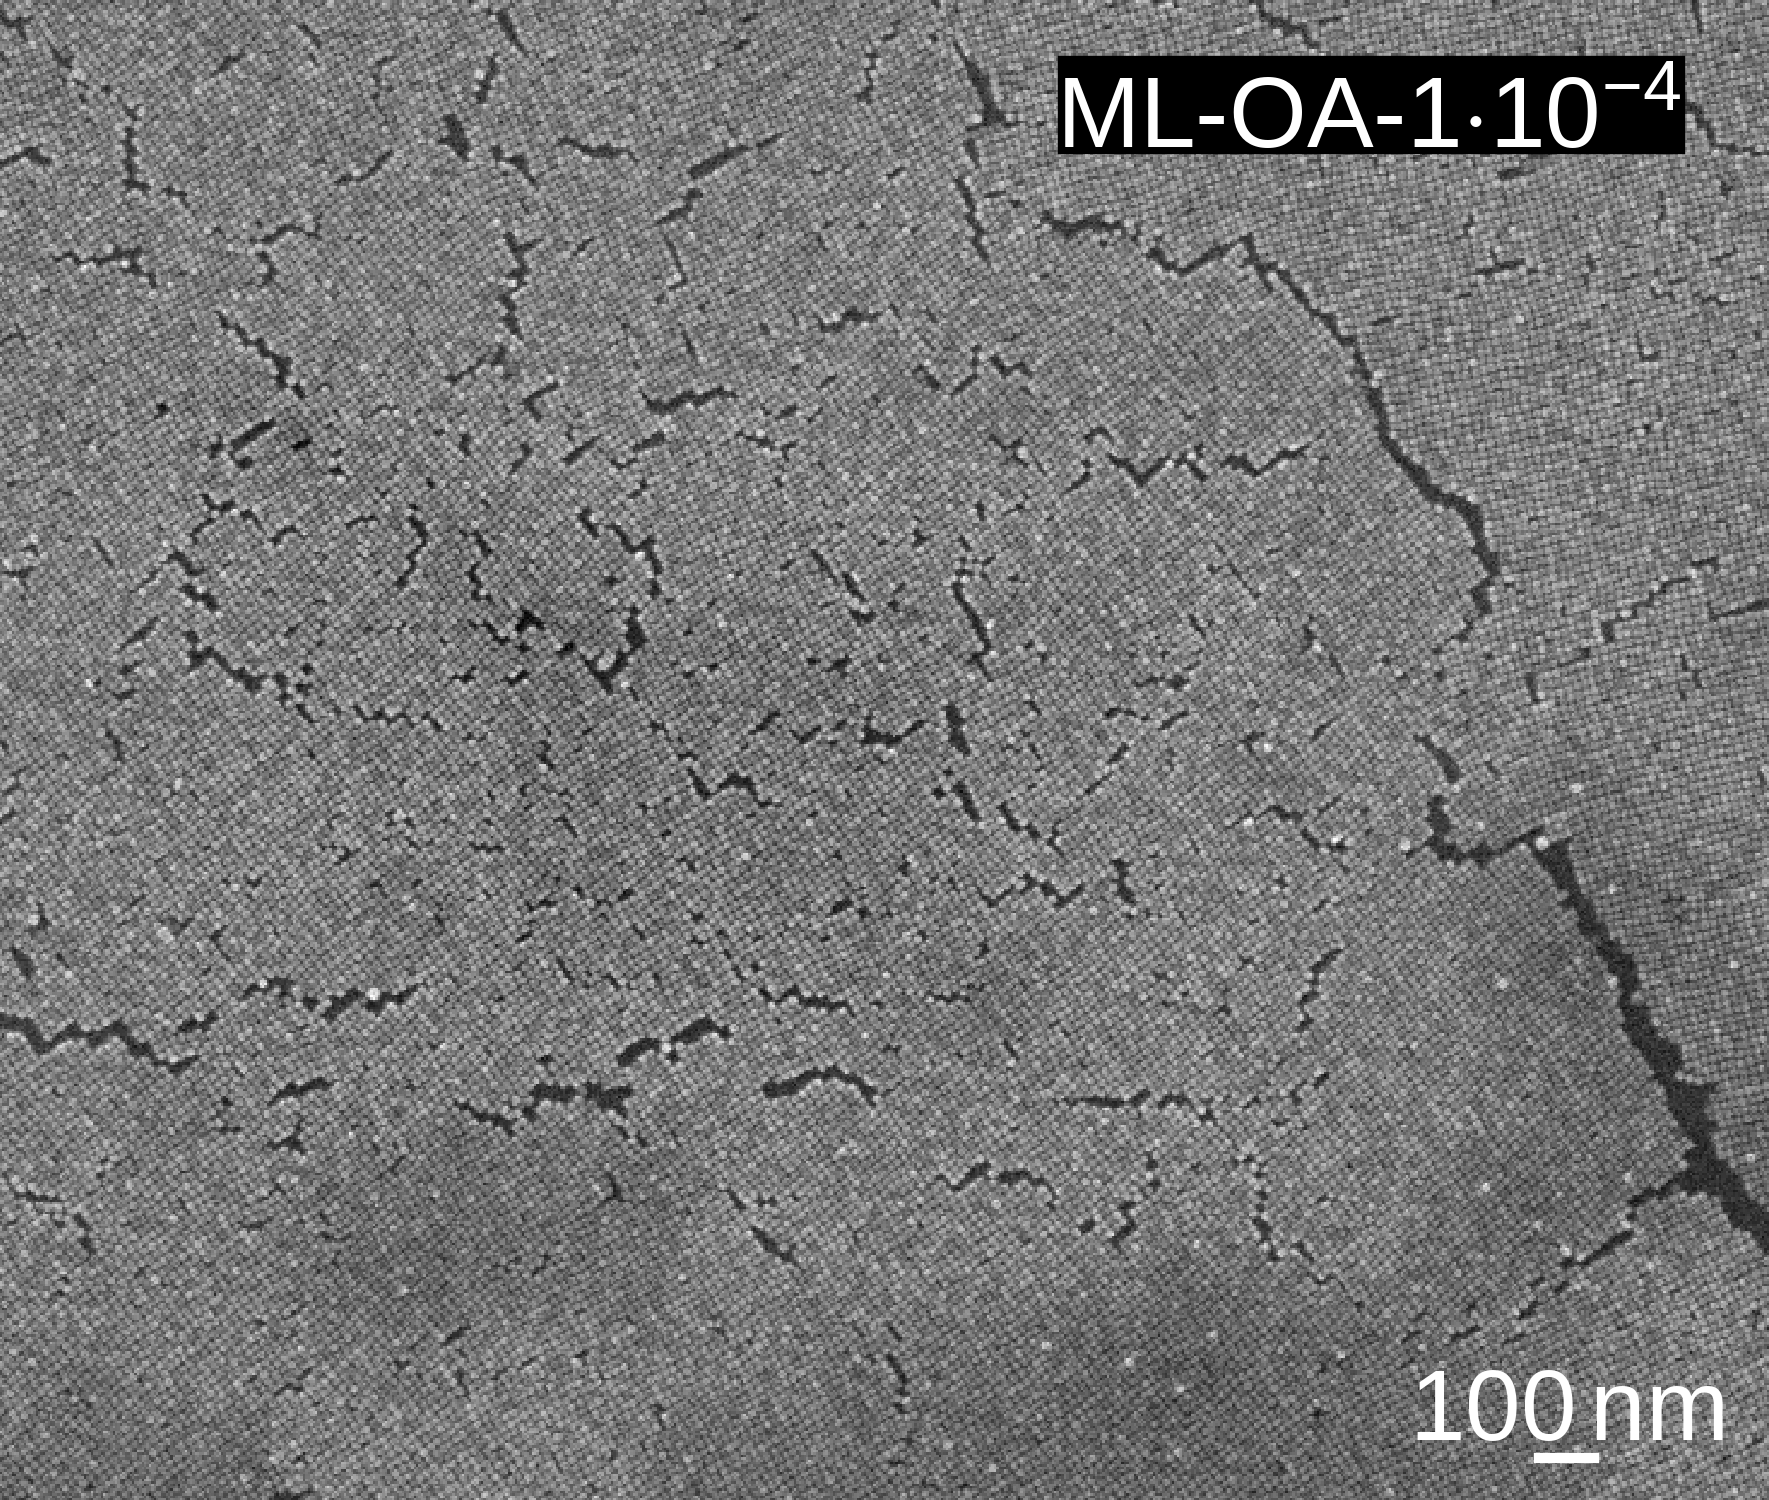
\includegraphics{monolayers_SEM_ML-OA-1e-4}
    \caption{\label{fig:monolayers:preparation:solventVariation:OAAddend}Variation of the oleic acid content analyzed in scanning electron microscopy. Monolayers drop casted from a dispersion of cobalt ferrite nanocubes with $5\cdot10^{-4} \unit{\%}$ (upper left), $1\cdot10^{-3} \unit{\%}$ (upper right), $5\cdot10^{-3} \unit{\%}$ (lower left) and $1\cdot10^{-2} \unit{\%}$ (lower right) oleic acid addend in the dispersion are shown.}
  \end{figure}

  To verify this assumption, a \textit{n}-heptane/1-octadecene dispersion of cobalt ferrite nanocubes, prepared following the the acetylacetonate route, is prepared with a particle concentration of $c_m \eq 0.12 \unit{mg/mL}$ and a 1-octadecene content of $2\unit{\%}$.
  Then, varied amounts of oleic acid are added to the particle dispersion and $V_\textsf{disp} \eq 50 \unit{\unitmu L}$ are drop casted on a clean silicon wafer of $ A_\textsf{wafer} \eq 1 \times 1 \unit{cm^2}$ size.
  The resulting structures are analyzed qualitatively in SEM with exemplarly images shown in \reffig{fig:monolayers:preparation:solventVariation:OAAddend}.
  The images clearly show the trend for increasing long order conditions with increasing the oleic acid content above $c_V^\textsf{OA} \eq 5\cdot10^{-3} \unit{\%}$.
  To put this amount into context, one can estimate which height the oleic acid film would have if it is evenly distributed on the silicon wafer surface by
  \begin{align}
    h \eq \frac{c_V^\textsf{OA} V_\textsf{disp}}{A_\textsf{wafer}}, \label{eq:monolayers:preparation:solventVariation:OAAddend}
  \end{align}
  to $h \eq 25 \unit{nm}$.
  Thus, the needed amount of oleic acid addend within the dispersion to obtain a monolayer formation has as order of magnitude about 2-3 times the nanoparticle size.
  One is limited in the amount that one adds to the dispersion as oleic acid is very difficult to remove from the wafer after the drying of the primary solvent and the 1-octadecene and therefore should be kept minimal.
  It is reasonable to assume that the additional oleic acid during the final drying stage functions as a thin mobilization layer on which the nanocubes can still move in two dimensions, rearrange and reduce the defects in the lattice.

  In summary, the presented data show that a combination of \textit{n}-heptane, 1-octadecene and oleic acid, with fine-tuned ratios, lead to long-range order for oleic acid capped nanoparticles into two dimensional structures that depend on the particle shape.
  It is however important that more parameters are considered during and after the two drying stages to obtain clean and homogeneous monolayers, as is discussed in the following.

\end{document}